\documentclass[UTF8]{ctexart}
\usepackage{amsmath}
\usepackage{graphicx}
\usepackage{float}
\usepackage{subfigure}
\usepackage{xeCJK}
\usepackage{hyperref}
\usepackage{algorithm2e}
\usepackage{amsfonts}
\usepackage{epsfig}
\usepackage{listings}

\graphicspath{{images/}}
\setCJKmonofont{Microsoft YaHei}

{}\title{\Huge{数学建模实验第一次作业\\初识mathematica}}
\author{\Huge{易凯}}
\date{\Huge{\today}}

\begin{document}
	\maketitle
	\vspace{35mm}
	\begin{flushright}
	\Large{
  	\textbf{班级} \makebox[5em][l]{软件53班}

  	\textbf{学号} \makebox[5em][l]{2151601053}

  	\textbf{邮箱} \makebox[5em][l]{williamyi96@gmail.com}

  	\textbf{联系电话} \makebox[5em][l]{13772103675}

  	\textbf{个人网站} \makebox[5em][l]{https://williamyi96.github.io}

  	\textbf{提交日期} \makebox[5em][l]{\today}
  	}
  	\end{flushright}
  	\newpage
  	\tableofcontents
	  \newpage

  \section{mathematica语言使用以及使用心得}
  \subsection{mathematica语言概述}
  \paragraph{1) 基本情况说明}

  ~

  mathematica是等同于matlab的可以高效进行复杂的数值以及矩阵运算的软件包,其内容丰富、功能齐全、操作简单、使用方便。同时其还支持与其他语言的交互使用。虽然mathematica是非免费的软件包,但是在中国的特殊国情之下,享受正版的mathematica应用还是不存在多大问题的。因此以下所有内容都是在mathematica5.0的环境下进行执行的。

  \paragraph{2) 命令的输入与运行}

  ~
  
  \begin{figure}[!htb]
  \centering
  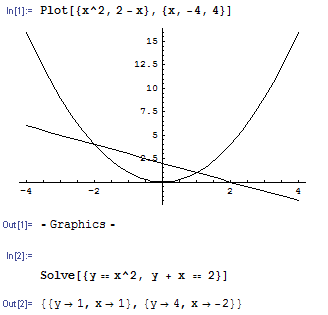
\includegraphics[]{1.png}
  \end{figure}

  最简单而且最为典型的例子就是画出曲线并且求出曲线之间的交点。其中曲线的绘制使用Plot指令,其参数为两条曲线的显函数和定义域的取值范围。求出曲线的交点使用Solve指令,其参数为对应的两个函数。值得注意的是,上述两条指令为首字母大写。
  
  \paragraph{3) 程序的保存与调用}

  ~

  全部文件的保存较为简单,如果我们需要保存程序的部分内容,则可以使用“表达式>>文件名.m”的格式进行。

  \begin{figure}[!htb]
  \centering
  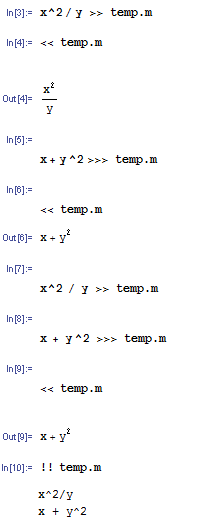
\includegraphics[]{2.png}
  \end{figure}

  \begin{figure}[!htb]
  \centering
  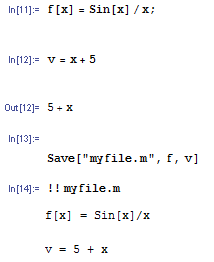
\includegraphics[]{3.png}
  \end{figure}

  以上表示了文件的两种不同的片段化保存形式。其中,>>命令直接保存,然后可以通过!!<文件名>查看相关内容,使用>><文件名>查看最后一次内容记录。Save可以保存之前的代码片段,调用方式同上。

  \subsection{初等数学之数值计算}
  mathematica的数值计算的精度理论上可以达到任意精度,但是若数据过大,其仍然会有溢出的可能性,如2\^1000000000。因此,我们如果想要一个近似值时,要么使用小数点,要么使用其相应的近似函数: N[expr] or expr\/\/N or N(expr, n)。前两个函数精度为6,最后一个函数保留至n位精度。

  关于数学函数以及常数的相关内容,详情可以参照教材,Pi,E,I, Infinity是需要重点记忆与掌握的内容。
  
  \subsection{符号计算}
  符号计算也就是代数式的计算,同样也是mathematica的重要功能。具体细节可以参照书本。
  值得注意的是以下情况:

  x=value //resign the value to x

  x=. //clear the value in x

  expr/.x-> value //replace x in expr by value

  expr/.{x->xvalue, y->yvalue}  //replace x and y in expr by xvalue and yvalue respectively

  关于其具体代数运算的操作参见书本。

  \subsection{微积分与线性代数}
  对于高等函数中的数值计算等问题,mathematica强大的软件包依然可以得到很好的求解,关于其具体的语法参见课本。

   
  \subsection{绘图}
  mathematica可以绘制平面图形以及三维图形,关于其具体的绘图操作之后进行系统归纳。


  \subsection{mathematica应用实例}
  \paragraph{1). 圆周率Pi的计算}

  ~

  \textbf{1.1 利用圆的面积计算}

  将圆分为四个部分,同时每个部分将其分割为曲边梯形进行逼近求解。
  
  \begin{figure}[!htb]
  \centering
  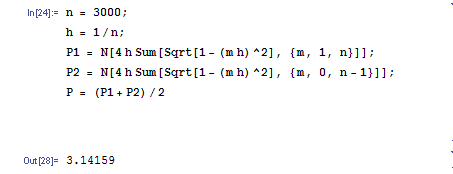
\includegraphics[]{4.1.png}
  \end{figure}

  \textbf{1.2 数值计算法}
  
  \begin{figure}[!htb]
  \centering
  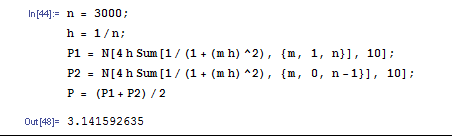
\includegraphics[]{4.2.png}
  \end{figure}

  值得注意的是,使用此方法在n大小相同时,计算结果的精度明显得到了提高。同时注意其使用方法。

  \textbf{1.3 无穷级数法}

  贴反正切函数的公式或者是三角公式,解决方法同上,只是提供了一种额外的思路而已。

  \paragraph{2). 供煤方案}
  供煤方案问题是一个典型的线性规划问题,因此也就是在约束条件之下求最小值的问题。

  \subsection{mathematica使用总结}
  \paragraph{mathematica性能优势}

  ~

  总体而言,mathematica的性能十分强大,特别是其对于数值计算的支持,为非专业程序员实现数值计算问题带来了巨大的便利,同时其特别注重对于英文文法的贴近,因此不像有C、Cpp、Java等半用户友好,半计算机友好的语法,其高度继承化,同时主要的适用对象是用户,因此相对而言其还是很好上手的。

  \paragraph{mathematica使用当中收获}

  ~

  在使用mathematica进行书上习题的演算时,明显感受到了其计算能力的强大,同时也体会到了其数值计算的突出性能,其高度继承化的英文文法式函数库的调用,为解决复杂的问题提供了一种简便的但是行之有效的方式。总体而言,同MATLAB一样,其能力还是挺不错的。

  \paragraph{后期使用感想}
  
  ~

  从mathematica的官网上了解到,虽然是学生用户,但是实际上还是需要200美元,同时该软件包的总大小为2.83G, 而且有严格的MD5码限制,不允许使用第三方p2p软件进行快速下载,虽然我有mathematica 11破解机,但是要让我下上两天,我也是不愿意的。因此,就此处的用户体验而言,差评。今后,我只用MATLAB,如果没有很强烈的需求,我再也不用mathematica了,毕竟MATLAB 8G的下载大小不是吃素的,mathematica能干的事情它都能干。

  \section{实际应用程序}
  \subsection{基本说明}
  由于相对而言,自己是数学建模的初学者,所以不是特别注重数学建模论文写作的格式,因此以写作业的形式来表述对应的题目。另外,由于时间关系,对于该题目的推广不能够达到很好的水准,之后如果有时间会继续进行深入的研究。

  \subsection{题目描述}
  \paragraph{棋子的颜色变化问题:}

  任意拿出黑白两种颜色的棋子共8个,排成彼此相连的一个圆圈,然后在两颗颜色相同的棋子中间放一颗黑色棋子,在两颗颜色不同的棋子中间放一颗白色棋子,放完后撤掉原来所放的棋子,再重复以上过程。这样放下一圈后就拿走上次的一圈棋子,问这样重复进行下去各棋子的颜色会怎样变化。

  \subsection{题目分析}
  该题目如果建立数学模型就类比于数学中的正负数相乘,两个相同符号的数相乘始终为整数,两个相异符号的数相乘始终为负数。因此,我们可以将黑色棋子初始化为+1,白色棋子初始化为-1。然后分析经过上述过程一定 次数之后,正负数的情况(也就是棋子的颜色变化)。

  \subsection{解题步骤}
  首先,设初始状态的棋子排列分别为$a_1\ a_2\ a_3\ a_4\ a_5\ a_6\ a_7\ a_8\ a_1\ a_i\in {+1,-1}$。

  然后在每两个棋子中间,以乘法的形式进行插入,则得到了

  $a_1a_2\ a_2a_3a\ a_3a_4\ a_4a_5\ a_5a_6\ a_6a_7\ a_7a_8\ a_8a_1$.

  反复迭代上述过程,最后得到: 

  $a_1a_2^8a_3^28a_4^56a_5^70a_6^56a_7^28a_8^8a_1\ ... \ a_8a_1^8a_2^28a_3^56a_4^70a_5^56a_6^28a_7^8a_8$。

  因此,在重复上述代换8次之后,得到的每一位的数字均为1,由之前定义的法则可知,最终8枚无论怎样的棋子,最多经过8次变换,所有棋子都会转变为黑色。得证。

  \subsection{思考感想}
  上述过程实际上可以说是体现了数学中“建模”的精髓,其解题过程巧妙但是却趣味盎然,棋子颜色的问题的引申版本是:如果棋子的总数为2的n次方个,规则同上,试说明棋子最终呈现出来的状态。

  由于时间原因,暂时没有找到一条简单但是可以有效解决上述问题的思路,因此暂时不进行深入研究,在之后的数学建模学习中,如果想到了很好的解决方案,会马上对此次作业进行更新。
\end{document}